% These slides originally from Paul Goldsmith-Pinkham: https://github.com/paulgp

\documentclass[11pt]{article}
\usepackage[top=0.8in, bottom=0.78in, left=0.87in, right=0.87in]{geometry}
\usepackage{setspace}
\usepackage[T1]{fontenc}
\usepackage{times}
\usepackage{booktabs}
\usepackage{rotating}
\usepackage{graphicx}
\usepackage[section]{placeins} %Placeins.sty keeps floats `in their place', preventing them from floating past a "\FloatBarrier" command into another section.  To use it, declare "\usepackage{placeins}" and insert "\FloatBarrier" at places that floats should not move past, perhaps at every "\section".  
\usepackage[large, bf]{caption}
\usepackage[FIGTOPCAP]{subfigure}
\usepackage{pdfpages}
\usepackage{palatino}
\usepackage{pdflscape}
\usepackage{textcomp}
\usepackage{longtable}
\usepackage{nicefrac}
\usepackage{adjustbox}	% to adjust the size of objects to fit into a page
\usepackage[hyphens]{url}

\usepackage{natbib}
\bibpunct{(}{)}{;}{a}{,}{,}

\def\citeapos#1{\citeauthor{#1}'s (\citeyear{#1})}

%zero spacing between references
%\usepackage{bibspacing}
%\setlength{\bibspacing}{\baselineskip}

%%-----------------------------------------------------------------
%%Header
%\usepackage{fancyhdr}
%\fancyhf{}
%\fancyhead[C]{\textit{Preliminary and Incomplete}}
%\fancyfoot[C]{\thepage}
%\renewcommand\headrulewidth{0pt}
%\pagestyle{fancy}
%%-----------------------------------------------------------------

%\onehalfspacing
\doublespacing

\usepackage{amsmath, amsfonts, amssymb, amsthm}

%\usepackage{mathpazo} %Use Palotino fonts
\parskip 0ex  %Vertical distance between paragraphs, in "ex"s
\parindent 20pt

%\usepackage{harvard}
%\bibliographystyle{apsr}
%\bibliographystyle{dcu}

\usepackage[pdftex]{hyperref}
\hypersetup{colorlinks, citecolor=blue, filecolor=blue, linkcolor=blue, urlcolor=blue}

\newtheorem{theorem}{Theorem}
\newtheorem{lemma}{Lemma}
\newtheorem{proposition}{Proposition}
\newtheorem{corollary}{Corollary}
\newtheorem{prediction}{Prediction}
\newtheorem{case}{Special Case}

\newenvironment{proofAlt}[1][Proof]{\begin{trivlist}
\item[\hskip \labelsep {\bfseries #1}]}{\end{trivlist}}
\newenvironment{definition}[1][Definition]{\begin{trivlist}
\item[\hskip \labelsep {\bfseries #1}]}{\end{trivlist}}
\newenvironment{example}[1][Example]{\begin{trivlist}
\item[\hskip \labelsep {\bfseries #1}]}{\end{trivlist}}

\newenvironment{remark}[1][Remark]{\begin{trivlist}
\item[\hskip \labelsep {\bfseries #1}]}{\end{trivlist}}
\def\urltilda{\kern -.15em\lower .7ex\hbox{\~{}}\kern .04em}

\renewcommand{\thesubfigure}{(\Alph{subfigure})}

%%%%%%%%%%%%%%%%%%%%%%%%%%%%%%%%%%
% SPACING
%%%%%%%%%%%%%%%%%%%%%%%%%%%%%%%%%%

\usepackage{titlesec}

\titlespacing*{\section}{0pt}{1.5ex plus 1ex minus .2ex}{0.8ex plus .2ex}
\titlespacing*{\subsection}{0pt}{1.2ex plus 1ex minus .2ex}{0.8ex plus .2ex}
% Decimal align 
\usepackage{dcolumn}
\newcolumntype{d}[0]{D{.}{.}{5}}

\usepackage{graphicx}
\graphicspath{{../../output/}}
\usepackage[]{epstopdf}
% This adds the output directory to the inputs function (code outputs are latex inputs!) so you don't have to use a relative path each time
\makeatletter
\providecommand*{\input@path}{}
\g@addto@macro\input@path{{../../output/}}% append
\makeatother


\usepackage[space]{grffile}

 
\title{\textbf{\LARGE{PAPER TITLE}}\thanks{First version: DATE. This version: \today.  ACKNOWLEDGEMENTS HERE}}

\author{
	AUTHOR 1\thanks{UNIVERSITY 1. Email: \href{mailto:author@address.com}{author@address.com}} \and
	AUTHOR 2\thanks{UNIVERSITY 2. Email: \href{mailto:author@address.com}{author@address.com}} \and 
	AUTHOR 3\thanks{UNIVERSITY 3. Email: \href{mailto:author@address.com}{author@address.com}} \and 
	AUTHOR 4\thanks{INSTITUTION 1. Email: \href{mailto:author@address.com}{author@address.com}} 
	}
			
\date{\today}

\begin{document}

\maketitle
\thispagestyle{empty} 
\setcounter{page}{0}

\begin{abstract}
ABSTRACT HERE

\end{abstract}


	  
%%%%%%%%%%%%%%%%%%%%%%%%%%%%%%%%%
% Text
%%%%%%%%%%%%%%%%%%%%%%%%%%%%%%%%%
	
\clearpage

The model is:
$$
\begin{aligned} 
	\vec{y}_t & = \Gamma \vec{f}_t + \vec{u}_t \\ 
        \vec{f}_t & = A_1 \vec{f}_{t-1} + A_2\vec{f}_{t-2} + \Xi_t \quad \quad \Xi_t \thicksim \mathcal{N}(0,I)\\ 
	 \vec{u}_t  & = B_1 \vec{u}_{t-1} + B_2\vec{u}_{t-2} + \Phi_t \quad \quad \Phi_t \thicksim \mathcal{N}(0,\Sigma)
\end{aligned} 
$$
where capital Greek and Latin characters represent matrices, arrows over characters denote vectors, and it is assumed that the different components of the `innovations' in the error updating equation are uncorrelated so that $ \Sigma $ is a diagonal matrix. The model has one unobserved factor that follows an AR(2), and the errors similarly follow an AR(2).

\begin{center}
\begin{tabular}{lclc}
\toprule
\textbf{Dep. Variable:}          & ['emp', 'gdp', 'hhc', 'iop', 'ios'] & \textbf{  No. Observations:  } &                 355                  \\
\textbf{Model:}                  &  DynamicFactor(factors=2, order=2)  & \textbf{  Log Likelihood     } &              -2122.477               \\
\textbf{}                        &            + AR(2) errors           & \textbf{  AIC                } &               4310.955               \\
\textbf{Date:}                   &           Thu, 09 Jan 2020          & \textbf{  BIC                } &               4438.735               \\
\textbf{Time:}                   &               23:13:06              & \textbf{  HQIC               } &               4361.789               \\
\textbf{Sample:}                 &              04-30-1990             & \textbf{                     } &                                      \\
\textbf{}                        &             - 10-31-2019            & \textbf{                     } &                                      \\
\bottomrule
\end{tabular}
\begin{tabular}{lcccccc}
                          & \textbf{coef} & \textbf{std err} & \textbf{z} & \textbf{P$>$$|$z$|$} & \textbf{[0.025} & \textbf{0.975]}  \\
\midrule
\textbf{loading.f1.emp}   &       7.7198  &        1.081     &     7.143  &         0.000        &        5.602    &        9.838     \\
\textbf{loading.f2.emp}   &      -0.5070  &        0.428     &    -1.184  &         0.236        &       -1.346    &        0.332     \\
\textbf{loading.f1.gdp}   &       4.4642  &        0.332     &    13.441  &         0.000        &        3.813    &        5.115     \\
\textbf{loading.f2.gdp}   &       0.2476  &        0.232     &     1.065  &         0.287        &       -0.208    &        0.703     \\
\textbf{loading.f1.hhc}   &       2.2967  &        0.334     &     6.873  &         0.000        &        1.642    &        2.952     \\
\textbf{loading.f2.hhc}   &       0.0905  &        0.122     &     0.740  &         0.459        &       -0.149    &        0.330     \\
\textbf{loading.f1.iop}   &       2.0257  &        0.382     &     5.297  &         0.000        &        1.276    &        2.775     \\
\textbf{loading.f2.iop}   &       0.0417  &        0.112     &     0.371  &         0.710        &       -0.178    &        0.262     \\
\textbf{loading.f1.ios}   &      12.7989  &        0.806     &    15.881  &         0.000        &       11.219    &       14.378     \\
\textbf{loading.f2.ios}   &       0.6643  &        0.659     &     1.008  &         0.314        &       -0.628    &        1.957     \\
\textbf{sigma2.emp}       &       0.0367  &        0.294     &     0.125  &         0.901        &       -0.540    &        0.613     \\
\textbf{sigma2.gdp}       &       0.0303  &        0.004     &     7.658  &         0.000        &        0.023    &        0.038     \\
\textbf{sigma2.hhc}       &       0.1247  &        0.007     &    18.216  &         0.000        &        0.111    &        0.138     \\
\textbf{sigma2.iop}       &       0.4116  &        0.026     &    15.985  &         0.000        &        0.361    &        0.462     \\
\textbf{sigma2.ios}       &       0.0225  &        0.020     &     1.122  &         0.262        &       -0.017    &        0.062     \\
\textbf{L1.f1.f1}         &       0.7897  &       26.066     &     0.030  &         0.976        &      -50.299    &       51.878     \\
\textbf{L1.f2.f1}         &       0.0331  &        1.871     &     0.018  &         0.986        &       -3.634    &        3.700     \\
\textbf{L2.f1.f1}         &       0.0284  &       31.461     &     0.001  &         0.999        &      -61.634    &       61.691     \\
\textbf{L2.f2.f1}         &      -0.0108  &        1.917     &    -0.006  &         0.995        &       -3.769    &        3.747     \\
\textbf{L1.f1.f2}         &       0.2779  &        2.187     &     0.127  &         0.899        &       -4.009    &        4.564     \\
\textbf{L1.f2.f2}         &       0.3943  &        0.171     &     2.304  &         0.021        &        0.059    &        0.730     \\
\textbf{L2.f1.f2}         &      -0.1851  &        2.271     &    -0.081  &         0.935        &       -4.636    &        4.266     \\
\textbf{L2.f2.f2}         &       0.0310  &        0.194     &     0.160  &         0.873        &       -0.349    &        0.411     \\
\textbf{L1.e(emp).e(emp)} &       0.5036  &        2.372     &     0.212  &         0.832        &       -4.146    &        5.153     \\
\textbf{L2.e(emp).e(emp)} &       0.3334  &        2.111     &     0.158  &         0.875        &       -3.805    &        4.472     \\
\textbf{L1.e(gdp).e(gdp)} &       0.9721  &        0.128     &     7.624  &         0.000        &        0.722    &        1.222     \\
\textbf{L2.e(gdp).e(gdp)} &      -0.1488  &        0.119     &    -1.253  &         0.210        &       -0.382    &        0.084     \\
\textbf{L1.e(hhc).e(hhc)} &       0.9047  &        0.142     &     6.353  &         0.000        &        0.626    &        1.184     \\
\textbf{L2.e(hhc).e(hhc)} &      -0.0635  &        0.141     &    -0.450  &         0.653        &       -0.340    &        0.213     \\
\textbf{L1.e(iop).e(iop)} &      -0.1792  &        0.056     &    -3.222  &         0.001        &       -0.288    &       -0.070     \\
\textbf{L2.e(iop).e(iop)} &      -0.0587  &        0.053     &    -1.101  &         0.271        &       -0.163    &        0.046     \\
\textbf{L1.e(ios).e(ios)} &       0.2006  &        0.133     &     1.509  &         0.131        &       -0.060    &        0.461     \\
\textbf{L2.e(ios).e(ios)} &       0.7877  &        0.145     &     5.419  &         0.000        &        0.503    &        1.073     \\
\bottomrule
\end{tabular}
\begin{tabular}{lclc}
\textbf{Ljung-Box (Q):}          & 75.96, 61.07, 150.64, 50.14, 33.55 & \textbf{  Jarque-Bera (JB):  } & 3.70, 16.59, 325.28, 54.11, 1250.25  \\
\textbf{Prob(Q):}                &    0.00, 0.02, 0.00, 0.13, 0.75    & \textbf{  Prob(JB):          } &     0.16, 0.00, 0.00, 0.00, 0.00     \\
\textbf{Heteroskedasticity (H):} &    2.43, 2.38, 0.90, 1.28, 0.60    & \textbf{  Skew:              } &   0.22, -0.07, -0.02, -0.42, 0.80    \\
\textbf{Prob(H) (two-sided):}    &    0.00, 0.00, 0.58, 0.18, 0.01    & \textbf{  Kurtosis:          } &    3.23, 4.05, 7.69, 4.71, 12.05     \\
\bottomrule
\end{tabular}
%\caption{Statespace Model Results}
\end{center}

Warnings: \newline
 [1] Covariance matrix calculated using the outer product of gradients (complex-step). \newline
 [2] Covariance matrix is singular or near-singular, with condition number 3.19e+16. Standard errors may be unstable.
\begin{figure}[h]
	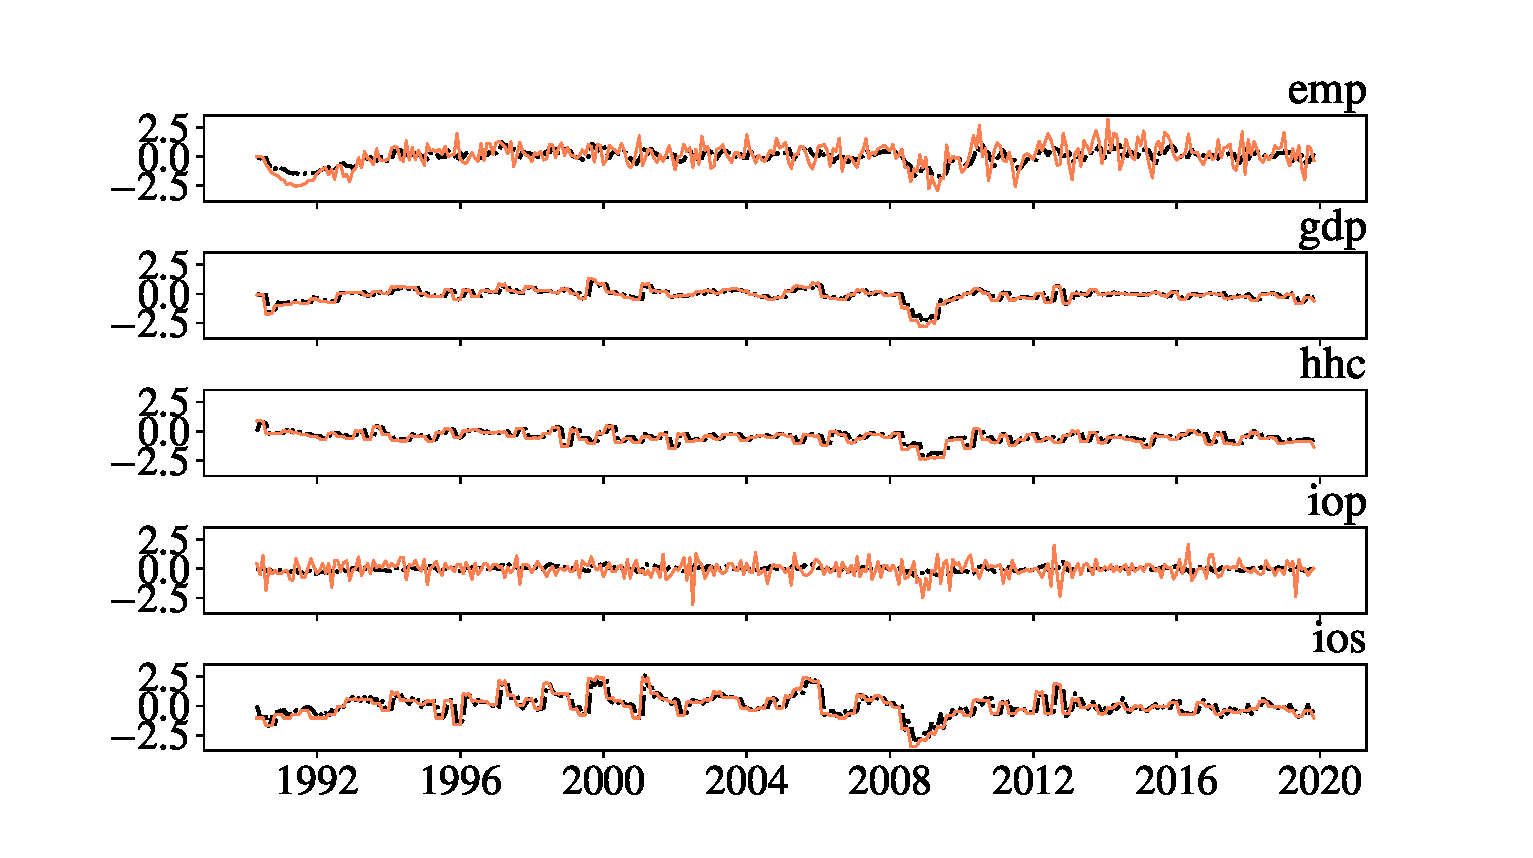
\includegraphics[width=\textwidth]{fcasts.eps} 
	\caption{Example figure. \label{fig:example}}
\end{figure}

\begin{figure}[h]
	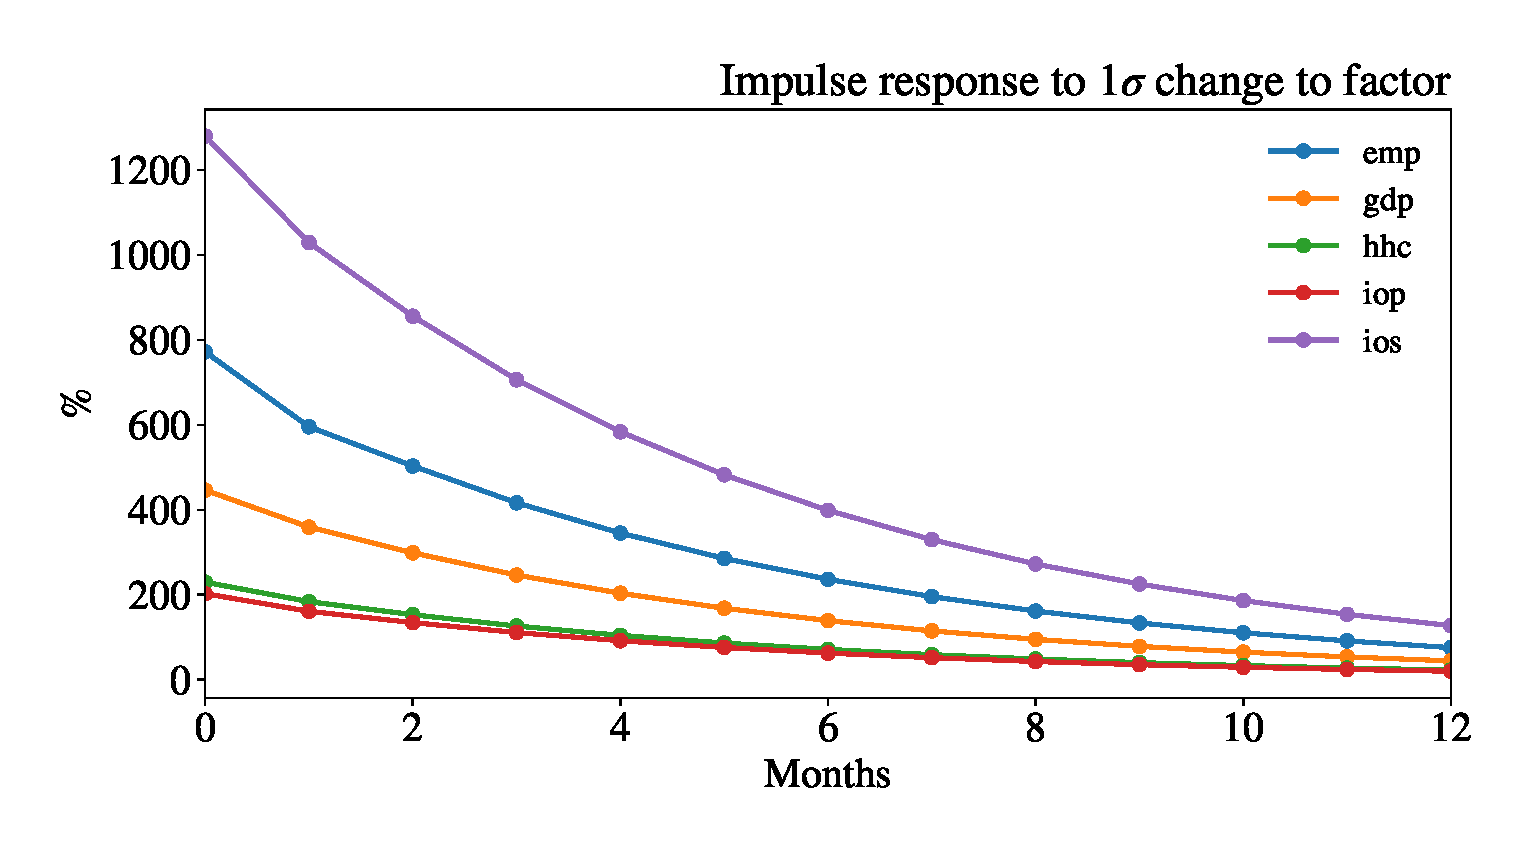
\includegraphics[width=\textwidth]{df_irfs.eps} 
	\caption{Example figure. \label{fig:example}}
\end{figure}

\newpage
\singlespacing 
\bibliographystyle{aea}
%\bibliography{bibliography.bib}

\onehalfspacing

%%%%%%%%%%%%%%%%%%%%%%%%%%%%%%%%%%
%%Figures and tables
%%%%%%%%%%%%%%%%%%%%%%%%%%%%%%%%%%

%\input{Figures.tex}
%\input{Tables.tex}

%%%%%%%%%%%%%%%%%%%%%%%%%%%%%%%%%
%Appendices
%%%%%%%%%%%%%%%%%%%%%%%%%%%%%%%%%

\clearpage  
\appendix

\renewcommand{\thefigure}{A\arabic{figure}}
\setcounter{figure}{0}

\renewcommand{\thetable}{A\arabic{table}}
\setcounter{table}{0}


\clearpage
\begin{center}
\vspace{-1.8cm}{\LARGE \textbf{PAPER TITLE}}\medskip \\
	\Large \textbf{Online Appendix} \bigskip \\
\large AUTHOR NAME 1 \hspace{0.3cm} AUTHOR NAME 2 \hspace{0.3cm} AUTHOR NAME 3 \hspace{0.3cm} AUTHOR NAME 4 \bigskip
	
\end{center}


%\input{Appendix_text.tex}

%\clearpage
%\input{Appendix_figures.tex}

%\clearpage
%\input{Appendix_tables.tex}




\end{document}
